% Part V: physics (sections 11-12)
\addcontentsline{toc}{part}{Part V \quad Physics}
\section{From a ball in a valley to the stochastic Allen--Cahn equation}\label{sec:allencahn}

\subsection{Rolling downhill}\label{sec:langevin}

Picture a ball in thick honey on a landscape of height $V(x)$. It has no inertia: its velocity is the force,
\begin{equation}\label{eq:gradflow}
  \frac{\dd x}{\dd s}=-V'(x),
\end{equation}
where $s$ is time. This is a \emph{gradient flow}. Along it the height only goes down,
$\frac{\dd}{\dd s}V(x(s))=V'(x)\frac{\dd x}{\dd s}=-V'(x)^2\le0$, and the ball stops at a bottom. Our landscape is the
\emph{double well}
\begin{equation}\label{eq:doublewell}
  V(x)=\tfrac14(x^2-1)^2,
\end{equation}
with two valleys at $x=\pm1$ (height $0$) and a barrier at $x=0$ of height $1/4$ (Figure~\ref{fig:langevin}a).

\subsection{Adding random kicks}

Now let the honey be warm, so that molecules kick the ball at random. A \emph{Brownian motion} $W(s)$ is the
limit of a random walk with ever smaller, ever more frequent steps: its increments over disjoint time
intervals are independent and $W(s+\delta)-W(s)\sim\N(0,\delta)$. Its variance grows linearly with time, so its
displacement grows like $\sqrt\delta$, much faster than $\delta$ for small $\delta$ (this is why its paths are rough).
The \emph{Langevin equation} adds kicks of strength set by a \emph{temperature} $\Th$:
\begin{equation}\label{eq:langevin}
  \dd x=-V'(x)\dd s+\sqrt{2\Th}\,\dd W,\quad\text{meaning}\quad x_{n+1}=x_n-V'(x_n)\,\delta+\sqrt{2\Th\delta}\;z_n
\end{equation}
for small time steps $\delta$ and independent standard normal $z_n$. At low temperature the ball rattles in one
valley and only rarely jumps the barrier; the typical waiting time grows like $e^{\Delta V/\Th}$ with $\Delta V$ the
barrier height (the Arrhenius law). Figure~\ref{fig:langevin}b shows the hops at $\Th=0.15$.

\subsection{Where the ball spends its time}

Release many independent balls and follow their density $p(x,s)$. Probability is conserved, so the density
in an interval changes only by what flows across its ends: $\partial_sp=-\partial_xJ$, with $J$ the
\emph{probability current}. Two things make probability flow. The drift carries density $p$ at velocity $-V'$,
a current $-V'p$. The kicks spread it from crowded to empty places, a current $-\Th\,\partial_xp$ (Fick's law;
the coefficient $\Th$ is fixed by matching the spread of $\sqrt{2\Th}W$ with the heat equation of \S\ref{sec:fourier}).
Hence the \emph{Fokker--Planck equation}
\begin{equation}\label{eq:fp}
  \partial_sp=\partial_x\big(V'p\big)+\Th\,\partial_x^2p .
\end{equation}
At equilibrium nothing flows, $J=0$, i.e.\ $\Th p'=-V'p$, whose solution is
\begin{equation}\label{eq:gibbs1}
  \pi(x)=\frac{1}{\Zp}\,e^{-V(x)/\Th}.
\end{equation}
This is the \emph{Boltzmann--Gibbs} law: low energy is likely, and temperature sets how much the law cares
about energy (Figure~\ref{fig:langevin}c). The zero-current condition is the continuous form of detailed
balance \eqref{eq:detbal}: the Langevin dynamics is reversible.

\begin{figure}[h]\centering
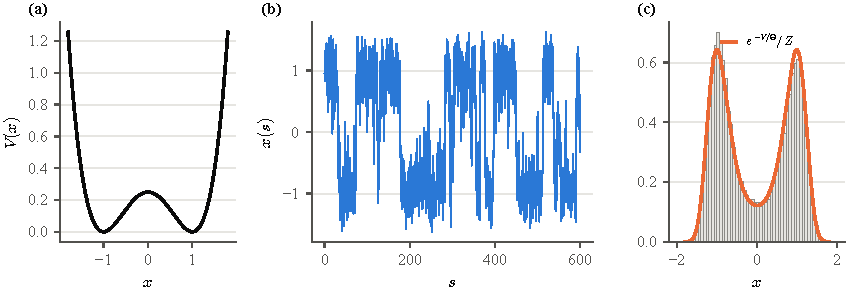
\includegraphics{primer-langevin.pdf}
\caption{(a) The double well $V$. (b) A Langevin path at $\Th=0.15$: long stays in a valley, rare hops. (c) The
histogram of the path against the Gibbs law $e^{-V/\Th}/\Zp$.}
\label{fig:langevin}
\end{figure}

\begin{keyidea}
The noising channel is a Langevin equation. With $V(x)=x^2/2$ and $\Th=1$, \eqref{eq:langevin} is the
Ornstein--Uhlenbeck process $\dd x=-x\dd s+\sqrt2\dd W$. Multiplying by $e^s$ gives $\dd(e^sx)=\sqrt2e^s\dd W$, so
started at $a$, $x(t)=e^{-t}a+\sqrt2\int_0^te^{-(t-r)}\dd W(r)$, a Gaussian with variance $2\int_0^te^{-2(t-r)}\dd r=1-e^{-2t}$.
That is exactly \eqref{eq:channel}. Its Gibbs law is $e^{-x^2/2}$, the standard normal, which is why pure noise
is where the channel ends.
\end{keyidea}

\subsection{From one ball to a string: where the Laplacian comes from}

Now take many balls, one at each point $x_i=ih$ of a line with spacing $h$, and call the value at point $i$
$\phi_i$ (think of $\phi_i$ as the local magnetisation, or the local composition of an alloy). Each $\phi_i$ sits in
its own double well, and neighbours are joined by springs that dislike differences. The total energy is
\begin{equation}\label{eq:latticeenergy}
  \En_h(\phi)=\sum_i\Big[\frac{(\phi_{i+1}-\phi_i)^2}{2h}+h\,V(\phi_i)\Big].
\end{equation}
The factors of $h$ make each piece represent a length $h$ of string: the spring term approximates
$\int\frac12(\partial_x\phi)^2\dd x$ and the well term $\int V(\phi)\dd x$. The derivative of $\En_h$ with respect to one value is
\[
  \frac{\partial\En_h}{\partial\phi_i}=-\frac{\phi_{i+1}-2\phi_i+\phi_{i-1}}{h}+h\,V'(\phi_i),
\]
and the second difference \eqref{eq:seconddiff} has appeared on its own: \emph{the springs pull each value towards
the average of its neighbours}. The gradient flow of the string, with each bead's force divided by the length
$h$ it represents, is
\begin{equation}\label{eq:latticeAC}
  \frac{\dd\phi_i}{\dd s}=\frac{\phi_{i+1}-2\phi_i+\phi_{i-1}}{h^2}-V'(\phi_i).
\end{equation}
As $h\to0$ the values become a function $\phi(x,s)$ of position and time (a \emph{field}; ``scalar'' only says
that its value at each point is a single number), the second difference becomes the second derivative in
space, and we get the \emph{Allen--Cahn equation}
\begin{equation}\label{eq:allencahn}
  \partial_s\phi=\partial_x^2\phi-V'(\phi).
\end{equation}
It is a \emph{partial differential equation} (PDE): an equation for a function of two variables involving its
derivatives in both. Two forces compete. The spring term is the heat equation: it smooths, pulling every
point towards its neighbours. The well term pushes every point towards $+1$ or $-1$. Allen and Cahn wrote it in
1979 for the separation of an alloy into regions of two phases.

\subsection{Kinks}

Where the field must change from $-1$ to $+1$ it forms a \emph{kink}. A kink at rest solves
\eqref{eq:allencahn} with $\partial_s\phi=0$: $\phi''=V'(\phi)$. Multiply by $\phi'$; the left side is the derivative of
$\tfrac12\phi'^2$ and the right side the derivative of $V(\phi)$, so $\tfrac12\phi'^2=V(\phi)$ (both vanish far from the
kink). Hence $\phi'=\sqrt{2V(\phi)}=(1-\phi^2)/\sqrt2$, which integrates to
\begin{equation}\label{eq:kink}
  \phi_{\rm kink}(x)=\tanh\big(x/\sqrt2\big),\qquad
  E_{\rm kink}=\int\Big[\tfrac12\phi'^2+V(\phi)\Big]\dd x=\int_{-1}^{1}\sqrt{2V(\phi)}\dd\phi=\frac{2\sqrt2}{3}\approx0.94 .
\end{equation}
The kink has width about $\sqrt2$ and costs a fixed energy $E_{\rm kink}$ (Figure~\ref{fig:field}a). A field made of
long stretches near $+1$ or $-1$ (\emph{domains}) separated by kinks is the typical low-temperature picture.

\subsection{Adding noise everywhere: the stochastic Allen--Cahn equation}

Heat the string: give every bead its own independent kicks, with strength scaled so that each piece of
string of length $h$ receives the right amount,
\begin{equation}\label{eq:sac}
  \dd\phi_i=\Big[\frac{\phi_{i+1}-2\phi_i+\phi_{i-1}}{h^2}-V'(\phi_i)\Big]\dd s+\sqrt{\frac{2\Th}{h}}\,\dd W_i .
\end{equation}
As $h\to0$ this is the \emph{stochastic} Allen--Cahn equation $\partial_s\phi=\partial_x^2\phi-V'(\phi)+\sqrt{2\Th}\,\eta$, with $\eta$
``space-time white noise'' (independent kicks at every point and every time). A PDE with random forcing is a
\emph{stochastic PDE}, an SPDE. In one space dimension this one is well defined: its solutions are continuous
but rough, like a Brownian path.

Where does the string spend its time? Exactly as for one ball. For any system $\dd X=-M\nabla\En\dd s+\sqrt{2\Th M}\dd W$
with a positive mobility $M$ ($M=1/h$ here), setting every component of the probability current to zero gives
\begin{equation}\label{eq:gibbsfield}
  p(\phi_1,\dots,\phi_L)\propto e^{-\En_h(\phi)/\Th}=\prod_i\exp\!\Big(-\frac{(\phi_{i+1}-\phi_i)^2}{2\Th h}\Big)\prod_i\exp\!\Big(-\frac{h\,V(\phi_i)}{\Th}\Big).
\end{equation}
\begin{keyidea}
The stationary law of the stochastic Allen--Cahn field on a lattice is \eqref{eq:gibbsfield}: a Gaussian random walk
in space (each step $\phi_{i+1}-\phi_i$ has variance $\Th h$) reweighted at every site by $e^{-hV(\phi_i)/\Th}$. Every factor
couples at most two neighbours. So by \S\ref{sec:bp} the spatial snapshot is a Markov random field on a line,
hence a Markov chain in the site index, and its exact denoiser is computable by belief propagation. We never
need to simulate the time dynamics \eqref{eq:sac}: the stationary law is all the data are drawn from.
\end{keyidea}

Two features of the lattice matter later. Each single step is \emph{nearly Gaussian} when $h$ is small, because
the reweighting factor $e^{-hV/\Th}$ is close to one; the non-Gaussian structure accumulates over the number of
sites spanned by a correlation length. And a fixed physical length contains more sites as $h$ shrinks, so a
denoiser that looks at a fixed number of neighbours sees a shrinking piece of physics.

\paragraph{Check yourself.}
\begin{enumerate}[label=\thesection.\arabic*,leftmargin=2.2em]
\item Verify that $\tanh(x/\sqrt2)$ solves $\phi''=V'(\phi)=\phi^3-\phi$.
\item What is the Gibbs law \eqref{eq:gibbs1} of the Langevin equation with $V(x)=x^2/2$ at temperature $\Th$?
\end{enumerate}

\section{The transfer operator: the field as a Markov chain}\label{sec:transfer}

\subsection{The transfer kernel and its spectrum}

Split each site factor of \eqref{eq:gibbsfield} evenly between the two bonds that touch it. The law becomes a
product of identical symmetric factors
\begin{equation}\label{eq:transfer}
  \mathsf T(\phi,\phi')=D(\phi)\,G(\phi'-\phi)\,D(\phi'),\qquad D(\phi)=e^{-hV(\phi)/2\Th},\quad G(u)=e^{-u^2/2\Th h}.
\end{equation}
Read $\mathsf T$ as an integral operator, $(\mathsf Tf)(\phi)=\int\mathsf T(\phi,\phi')f(\phi')\dd\phi'$; on a grid it is a symmetric matrix with
positive entries. By \S\ref{sec:toolbox} it has real eigenvalues $\lambda_0>\lambda_1\ge\lambda_2\ge\dots$, orthonormal
eigenfunctions $\psi_0,\psi_1,\dots$, and (Perron--Frobenius) a leading eigenfunction $\psi_0$ that is positive
everywhere. Integrating a long chain is applying $\mathsf T$ many times, so $\lambda_0$ and $\psi_0$ dominate.

\subsection{The ground-state transform}

Consider a site deep inside a long chain. Its marginal is the product of what the left half and the right half
say about it. Each half is $\mathsf T$ applied many times to the constant function at the far end, which by the power
method is proportional to $\psi_0$. So the stationary marginal is
\begin{equation}\label{eq:psi0sq}
  \pi(\phi)=\psi_0(\phi)^2\qquad(\textstyle\int\psi_0^2=1).
\end{equation}
Given the current site, the next one is drawn in proportion to the bond factor times everything to its
right, $\mathsf T(\phi,\phi')\psi_0(\phi')$ (the ``future factor'' of \S\ref{sec:futurefactor}). Normalising with the
eigen-equation $\int\mathsf T(\phi,\phi')\psi_0(\phi')\dd\phi'=\lambda_0\psi_0(\phi)$ gives the transition kernel
\begin{equation}\label{eq:gst}
  \boxed{\;K(\phi'\mid\phi)=\frac{\mathsf T(\phi,\phi')\,\psi_0(\phi')}{\lambda_0\,\psi_0(\phi)}\;}
\end{equation}
the \emph{ground-state transform} (the name comes from quantum mechanics, where $\psi_0$ is the lowest-energy
state). It is reversible with respect to $\pi=\psi_0^2$: $\pi(\phi)K(\phi'\mid\phi)=\psi_0(\phi)\mathsf T(\phi,\phi')\psi_0(\phi')/\lambda_0$ is
symmetric. Intuitively, $\psi_0(\phi')$ counts the good continuations available after arriving at $\phi'$.

\subsection{Correlations, and why there is no phase transition}

Insert the expansion $\mathsf T^r=\sum_n\lambda_n^r\psi_n\psi_n\T$ into the two-point function:
\begin{equation}\label{eq:corr}
  \E[\phi_i\,\phi_{i+r}]=\sum_{n\ge1}\Big(\frac{\lambda_n}{\lambda_0}\Big)^rc_n^2,\qquad c_n=\int\psi_0(\phi)\,\phi\,\psi_n(\phi)\dd\phi
\end{equation}
(the $n=0$ term is the squared mean, zero by symmetry). Correlations decay geometrically, dominated by
$\rho_1=\lambda_1/\lambda_0$, which plays the role of the AR(1) coefficient $\rho$: the correlation length is
$\xi=1/\log(\lambda_0/\lambda_1)$ sites. We fix the laboratory's second-order structure by choosing $h$ so that
$\rho_1=0.85$, the same value as the AR(1) laboratory.

Because $\lambda_0$ is strictly larger than $\lambda_1$ at every temperature, $\xi$ is finite: a one-dimensional system
never commits to one phase over an infinite length. The reason is entropy. A kink costs $E_{\rm kink}$ but can be
placed anywhere, so a long stretch always contains some, at a density that behaves like $e^{-E_{\rm kink}/\Th}$. The
domains are therefore long but finite, of length about $e^{E_{\rm kink}/\Th}$: a sharp crossover, not a phase
transition. Our frozen measurements (E32's fixed-spacing sweep) show coarse kink densities of $0.016$ and $0.066$
per unit length at $\Th=0.2$ and $0.3$, a ratio of $4.1$, against the Arrhenius ratio $e^{E_{\rm kink}(1/0.2-1/0.3)}=4.8$.

\begin{figure}[h]\centering
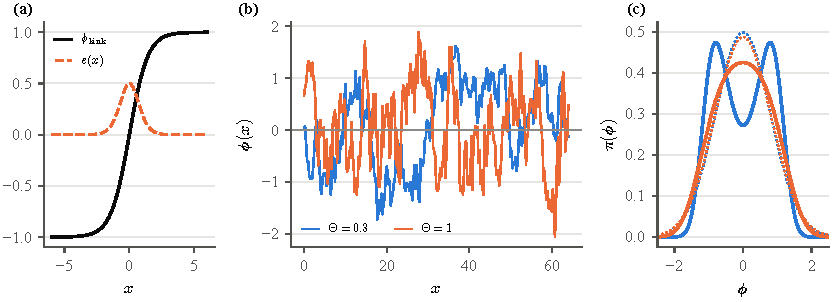
\includegraphics{primer-field.pdf}
\caption{(a) The kink $\tanh(x/\sqrt2)$ and its energy density, which integrates to $E_{\rm kink}=2\sqrt2/3$. (b) Exact
stationary fields at $h=0.25$ over a length of $64$: at $\Th=0.3$ (blue) long domains near $\pm1$ separated by kinks; at
$\Th=1$ (orange) a rough field that rarely settles. (c) The stationary marginal $\pi=\psi_0^2$ (solid) against the
Gaussian with the same variance (dotted): bimodal at $\Th=0.3$, already close to Gaussian at $\Th=1$.}
\label{fig:field}
\end{figure}

\subsection{Exact sampling and the numerics}

Since the chain is stationary with known $\pi$ and $K$, exact samples need no simulation in time: draw
$\phi_1\sim\pi$, then each next site from $K$. In the code, $\mathsf T$ is discretised on $2401$ points over $[-12,12]$, the
symmetric matrix $W^{1/2}\mathsf TW^{1/2}$ is diagonalised once per $(\Th,h)$, $\log\psi_0$ is interpolated by a spline,
and the field is standardised to unit variance, $a=\phi/s$ with $s^2=\Var_\pi\phi$, before the noise channel is applied.
The draw from $K$ is done by rejection: propose a Gaussian step of variance $\Th h$ and accept with probability
proportional to $\psi_0(\phi')D(\phi')$, a fact that the next chapter turns into a theorem.

\begin{caution}
The number of sign changes of a sampled field is \emph{not} its number of kinks. A rough path that crosses zero
once tends to recross it many times nearby, and on a finer lattice those recrossings multiply: the raw
sign-change density grows like $1/\sqrt h$ (measured: $0.120$, $0.175$, $0.247$ per unit length at $h=1,0.5,0.25$; N-31).
Counting only crossings that survive over a kink width ($\sqrt2$ in physical units) gives a statistic that agrees
across lattices within $11\,\%$, and across subsampling strides of one fine field within $8\,\%$ (E34, E36).
\end{caution}

\paragraph{Check yourself.}
\begin{enumerate}[label=\thesection.\arabic*,leftmargin=2.2em]
\item Check that the kernel \eqref{eq:gst} integrates to one over $\phi'$.
\item If $\lambda_1/\lambda_0=0.85$, after how many sites has the leading term of the correlation fallen below $0.1$ of its
  starting value?
\end{enumerate}
